\subsection{Voltage Supervisor (VS)}

The Voltage Supervisor Module (VS) keeps the \mu S in reset as long as the supply voltage
undershoots or overshoots the recommended operating conditions. When the master switches on
the slave power supply, a certain voltage drop is to be expected due to inrush current.
This drop increases as the battery charge decreases. Furthermore, the drop depends on the
ambient temperature. VS ensures that \mu S does not attempt to boot until
the supply voltage has recovered. Failing to do so could lead to undefined behavior.

\subsubsection{Requirements}

VS must be suitable for \SI{3.3}{\volt} systems.

\subsubsection{Implementation}


\begin{figure}[h]
    \centering
    \includegraphics[width=0.8\textwidth]{SL/VS/VS}
    % \caption{WD - schematic}
\end{figure}

\begin{table}[H]
    \centering
    \begin{threeparttable}[b]
        \begin{tabularx}{\linewidth}{ >
                    {\hsize=.25\hsize}X >
                    {\hsize=0.5\hsize}X >
                    {\hsize=.25\hsize}X  >
                    {\hsize=.5\hsize}X >
                    {\hsize=.25\hsize}X  >
                    {\hsize=3\hsize}X
            }
                  & \multicolumn{4}{c}{Pin mapping} &                                                                                      \\
            \cmidrule(lr){3-6}
            Id    & Net                             & Nb. & Name                          & Type            & Function                     \\
            \midrule
            $U_1$ & .3V3                            & 1   & \texttt{SENSE}                & \leftsquigarrow &                              \\
            $U_1$ & \Gnd                            & 2   & \texttt{GND}                  & \Gnd            &                              \\
            $U_1$ & \neg MR                         & 3   & \texttt{\textoverline{MR}}    & \leftharpoonup  & manual reset                 \\
            $U_1$ & .3V3                            & 4   & \texttt{VDD}                  & \leftarrow      &                              \\
            $U_1$ & CT                              & 5   & \texttt{CT}                   & \leftsquigarrow & adjustable reset  delay time \\
            $U_1$ & \neg RS                         & 6   & \texttt{\textoverline{RESET}} & \leftharpoonup  & reset output open drain      \\
        \end{tabularx}
    \end{threeparttable}
    % \caption{VS - pin mapping}
\end{table}
\begin{table}[H]
    \centering
    \begin{tabularx}{\linewidth}{>{\hsize=0.25\hsize}X
            >{\hsize=0.75\hsize}X >{\hsize=1.5\hsize}X
            >{\hsize=0.5\hsize}X >{\hsize=2\hsize}X}
        Id    & BOM Item                     & Order Code          & FF     & Rationale             \\
        \midrule
        $U_1$ & \cite{noauthor_tps3890_2016} & TPS389033DSER / 235 & WSON/6 &                       \\
        $R_p$ & \SI{10}{\kilo\ohm}           & generic             & 0603   &                       \\
        $C_t$ & \SI{100}{\nano\farad}        & generic             & 0603   & \SI{1}{\second} delay \\
    \end{tabularx}
    \caption{VS - BOM}
\end{table}
\clearpage